\documentclass{article}
\usepackage{amsmath}
% if you need to pass options to natbib, use, e.g.:
% \PassOptionsToPackage{numbers, compress}{natbib}
% before loading nips_2017
%
% to avoid loading the natbib package, add option nonatbib:
% \usepackage[nonatbib]{nips_2017}

%\usepackage{nips_2017}

% to compile a camera-ready version, add the [final] option, e.g.:
\usepackage[final]{nips_2017}

\usepackage[utf8]{inputenc} % allow utf-8 input
\usepackage[T1]{fontenc}    % use 8-bit T1 fonts
\usepackage{hyperref}       % hyperlinks
\usepackage{url}            % simple URL typesetting
\usepackage{booktabs}       % professional-quality tables
\usepackage{amsfonts}       % blackboard math symbols
\usepackage{nicefrac}       % compact symbols for 1/2, etc.
\usepackage{microtype}      % microtypography
\usepackage{subfig}
\usepackage{cleveref}
\usepackage{graphicx}
\usepackage{siunitx}

\usepackage{titlesec}

\setcounter{secnumdepth}{4}

\titleformat{\paragraph}
{\normalfont\normalsize\bfseries}{\theparagraph}{1em}{}
\titlespacing*{\paragraph}
{0pt}{3.25ex plus 1ex minus .2ex}{1.5ex plus .2ex}

\graphicspath{ {hw4/imgs/} }

\title{Computer Vision 1: Final Project}


\author{
	Gabriele Bani \\
	11640758 \\
  \texttt{gabriele.bani@student.uva.nl} \\
  %% examples of more authors
  \And
  	Andrii Skliar \\
  11636785 \\
  \texttt{andrii.skliar@student.uva.nl} \\
}

\begin{document}
\maketitle

\section{Introduction}
In this project we have analyzed two main approaches for image classification: Bag-of-Words approach and Convolutional Neural Networks approach.

We have analyzed Bag-of-Words classification approach with different settings, including various features for building visual vocabulary, different approaches to building visual vocabulary, namely K-Means clustering and Gaussian Mixture Models and different approaches for building image representation, such as histograms and Fisher vectors. We have tried various hyperparameters and have observed how they influence the performance of the algorithm. We have included detailed analysis of our results and possible ways of improving the algorithm.

We also analyze CNN architectures and understand their behavior under different hyperparameter settings. We explore how a pretrained network can be used on another dataset in order to achieve good results, without occurring in overfitting or underfitting behaviors, thanks to fine tuning procedures. We evaluate both qualitatively and quantitatively the features from the pre trained model and the fine tuned model, and show how fine tuning constantly produces superior results. Finally, we apply different additional variations to the training procedures and analyze their effects.  

\section{Bag-of-Words based Image Classification}
As mentioned in the task, Bag-of-Words based Image Classification system contains the following steps:

\begin{enumerate}
    \item Dataset formation
    \item Feature extraction and description
    \item Building a visual vocabulary
    \item Quantize features using visual dictionary (encoding)
    \item Representing images by frequencies of visual words
    \item Classification
\end{enumerate}

We would like to discuss each of the steps in detail and its implementation in the next section. 

\subsection{Implementation}
\subsubsection{Dataset formation}
Dataset is formed separately for training and testing phases. Firstly, vocabulary is constructed. To do so, we have used first 250 images per class.  Afterwards, out of all the images that are left, depending on the specified size, positive and negative training example are sampled for each class. It is done in a following way:
\begin{enumerate}
    \item Out of images, which were not used for the vocabulary, first $M$ (given number of positive examples) images are taken. Afterwards, we randomly sample $K$ (given number of negative examples) images 3 more times (generally, $N - 1$, where $N$ is the number of classes) to form negative examples of current class for all the other classes. This gives us $M + 3 * K$ (with $M$ being number of positive examples, $K$ - negative) number of images sampled (note, that they should not be unique) per class. 
    
    After repeating this procedure for each class, we get following matrix (here for a better understanding of the data structure being used): \begin{bmatrix}
    pos\_class\_1 & neg\_for\_class\_2 & neg\_for\_class\_3 & neg\_for\_class\_4\\
    pos\_class\_2 & neg\_for\_class\_1 & neg\_for\_class\_3 & neg\_for\_class\_4\\
    pos\_class\_3 & neg\_for\_class\_1 & neg\_for\_class\_2 & neg\_for\_class\_4\\
    pos\_class\_4 & neg\_for\_class\_1 & neg\_for\_class\_2 & neg\_for\_class\_3\\
    \end{bmatrix}
    \item We are transforming the matrix in order to have all positive and negative examples for one class in the same row.
\end{enumerate}

This procedure of dataset formation allows us for more robust work of the system as we are not dependent on the number of classes and can use our classifier to train on any new dataset. Note, however, that for this dataset, if we use 250 images for the vocabulary, we can only use maximum 150 images for the training purposes as class with the lowest amount of images consists of 400 images. Also, we didn't try to use different number of images per class in the same experiment as that might lead to class imbalance thus giving us worse results. However, it might be a good idea for a more extensive experimentation. 

\subsubsection{Feature extraction and description}
\label{feature_extraction}
There are two different options for feature extraction and description: regular SIFT, which extracts descriptors at each keypoint that it has found, and dense SIFT, which extracts descriptors at each k-th pixel. Both approaches are easy to implement using vlfeat functions. However, the main confusion here comes from the fact that SIFT has to be applied to images in different colorspaces. To do this, we have done following:
\begin{enumerate}
    \item (only for regular SIFT) Convert image to grayscale and find keypoints
    \item Calculate descriptors for each of the keypoints. Here, we have used vlfeat function vl\_siftdescriptor and have followed an example for calculating gradient provided in the vlfeat documentation page \footnote{\url{http://www.vlfeat.org/matlab/vl_siftdescriptor.html}}.
    \item Concatenate descriptors calculated at the same position along the first dimension over all color channels. Thus, in case of 3-channel image for each of the keypoints we will have a vector of size $128*3 = 384$.
    \item Vectors obtained in the previous step are being concatenated into one matrix and are used as a temporary image representation.
\end{enumerate}
Note, that this operation is done for each image in the formed dataset.
Also, one more issue that we have encountered is that some of the images in a dataset are grayscale. For that case, if we have encountered those, we copy single gray channel 3 times in order to form 3-channel image.
\subsubsection{Building a visual vocabulary}

To form a visual vocabulary, we apply clustering algorithm (in our case, K-means) to the images, which have been selected as a vocabulary set. After running K-means, we get matrix of size $K x 128*n_channels$, where $K$ is a number of clusters (size of the vocabulary) and $128*n_channels$ is a dimensionality of each feature. These will serve as visual words.

\subsubsection{Quantize features using visual dictionary (encoding)}

Afterwards, we need to calculate number of occurrences of these visual words in each image. To do so, for each feature extracted in step 2 (\cref{feature_extraction}), we find the closest visual word (thus, closest cluster) and represent it as an id of the closest cluster (thus, row number in the matrix of visual words). To do so, we have used very convenient matlab function dsearchn \footnote{\url{https://nl.mathworks.com/help/matlab/ref/dsearchn.html}}, which finds the index of the nearest point in N-dimensional space. This way, we represent image as an unordered list of visual words.

\subsubsection{Representing images by frequencies of visual words}

To get image representation in a form of frequencies of visual words, we calculate number of occurrences of each visual word in the image and normalize it by the total number of visual words in the image. This can be thought of as a histogram with as many bins as size of the vocabulary (number of clusters). So, now each image will look something like following: $(a_1, a_2, \ldots a_{K}) = (0, 0.01, 0.19, \ldots 0)$.

\subsubsection{Classification}

Before actually doing classification, we need to label data for each class. In our case, we label images of the correct class with 1 and other classes as -1. So, now for each training and testing example, we get following vector: $(a_1, a_2, \ldots a_K, label)$. 
After that, we apply the classification algorithm (One-vs-all SVM in our case) to the data. Generally, because our data is imbalanced (normally, $K$ positive examples and $3 * K$ negative examples), without carefully tuning the parameters, SVM performs pretty bad, simply predicting -1 thus getting an accuracy of $75\%$ for all the classes. To avoid that problem, we have automatically done parameter tuning using built-in tools of LIBSVM \footnote{\url{https://github.com/cjlin1/libsvm}} (\cite{libsvm}). \\
We are using 3 types of kernels: linear, polynomial and RBF. For all the kernels, we optimize cost parameter (in range $(2^{-5}, 2^{-4} \ldots 2^{-3})$), which is responsible for how strong we will penalize our SVM for actually misclassifying data. For polynomials and RBF, we also optimize gamma in the same range as cost. For polynomials we are also optimizing degree, which is the degree of a polynomial function that will be used. 
All the training is performed in a 10-fold cross-validation mode, which allows for more correct training without actually overfitting to the training data. So, we find the parameters, which give us the highest cross-validation accuracy, retrain it on the whole dataset and use them for testing our classifier. 
Note, that this is being done for each class and thus classifiers may use different hyperparameters for each class.

\subsection{Results and Discussion}

Here we would like to discuss the results that we have obtained. Due to the fact that an extensive grid search would take 5490 experiments (*3 for each kernel), we have chosen our baseline model, which we have used for testing different assumptions. As a baseline model for regular SIFT (not dense SIFT), which will be discussed first, we have chosen the one with 150 positive and 150 negative examples per class (so, 600 images in training set for each class), 400 clusters (size of vocabulary), gray-SIFT and linear kernel. For dense SIFT, we use 50 positive and 50 negative examples per class (so, 200 images in training set for each class), SIFT step size of 5 pixels, SIFT block size of 3 pixels and 400 clusters (size of vocabulary). For both options, number of examples used for training the vocabulary is 250.

\subsection{Vocabulary size}

First, we would like to discuss results obtained for different vocabulary size, presented in \cref{sift_vocab_results} and \cref{dense_vocab_results}. As we can see, mean average precision changes quite significantly depending on the vocabulary size. Even more importantly, average precision per class changes very significantly per class. It may be caused by several reasons, which we would like to discuss in more detail. 

As mentioned in \cite{visual_vocabulary_size}, in general there is no fixed optimal vocabulary size for the images and it highly depends on the data itself. Small visual vocabulary size results into multiple features being represented by one word in a vocabulary thus reducing the discriminative power of the classifier. At the same time, very large visual vocabulary size can add noise and therefore harm the performance of the classification. 

However, it is also important to understand that each classifier has been specifically optimized for the provided visual vocabulary, therefore it is difficult to reason about whether performance differs for different classes is due to those classes being more linearly separable in the latent space (and thus can be classified better using linear SVM or due to the size of the visual vocabulary). 

Also, it's important to notice that different vocabulary size might be more suitable for images of one class and less suitable for other classes due to the amount of actual discriminative features common for images of each class.

An interesting thing to see, however, is that larger size of the vocabulary (4000) performs better for dense SIFT and worse for the regular SIFT. This is most probably due to that dense SIFT finds many more descriptors than regular SIFT, so size of the vocabulary should be much bigger in order to account for larger amount of discriminative features.

\subsection{SIFT Colorspace}

Next, we would like to discuss effect of colorspaces on the final result. We have tried the following colorspaces: Grayscale, RGB, normalized RGB (written as rgb), opponent-RGB, HSV. We have visualized results in \cref{sift_colorspace_results} and \cref{dense_colorspace_results}. Similarly to the different vocabulary size, mean average precision differs significantly for various colorspaces. Again, we can see that depending on the target class, different colorspaces can be more suitable. There is no evident reason for better performance of one colorspace for specific class as the performance highly depends on the dataset itself. However, possible reasons will be discussed further. In our discussion we will mostly be using \cite{colorspaces} as it contains a lot of details about effects of different colorspaces on image recognition.

Grayscale colorspace was used as a baseline and it performs pretty well due to the SIFT properties: shift and scale invariance, light intensity change invariance, light intensity shift invariance, light intensity change and shift invariance, light color change invariance, light color change and shift invariance. 

Compared to grayscale-SIFT, both RGB-SIFT and rgb-SIFT lose illumination color invariance, with former also losing illumination intensity invariance, which might result in both better and worse performance depending on the dataset. This might consist of images taken under the same or very different lighting conditions, which will respectively make it better or worse. Notice however, that the main change compared to grayscale-SIFT is that SIFT descriptors are concatenated over all three channels thus resulting in more descriptive and possibly discriminative features.

Though \cite{colorspaces} reported opponent-SIFT to be working better than any other SIFT features, possibly due to the fact that it is not fully invariant to changes in light intensity and light color. However, for us it performs bad because of the single grayscale image in the set of Motorbike images. More specifically, because we convert it to 3-channel image by replicating its single channel, when converting to opponent-SIFT, first two layers will be zeroed out as suggested by formulas: $O1 = \frac{(R-G)}{\sqrt{2}}; O2 = \frac{(R+G-2B)}{\sqrt{6}}$, where $R, G$ and $B$ represent corresponding color channels and this possibly results in classifier not being able to handle this image correctly. 

Despite the main disadvantage of HSV-SIFT, which is that hue gets unstable under condition of low saturation and therefore gets ignored, HSV-SIFT performed best for us. Note, however, that it is not invariant to light color changes, as only V channel contains information about the intensity of the image and therefore is the only channel that is invariant to light color changes. Apparently, for our dataset the fact that it is only partially invariant was beneficial. However, as already mentioned, this is different from the results provided in \cite{colorspaces}, where OpponentSIFT performed best.

\subsection{Number of training examples}

You can see results for various number of training examples in \cref{num_examples}. However, as you can see, Mean Average Precision is pretty much the same (with difference of 1-2\%) for any number of examples. Therefore, the results suggest that an extensive search for good balance between positive and negative examples is not worth the improvement we can possibly get. Anyway, the tendency is clear: the more examples we use and the more balanced (where balanced means the same number of examples per class) the training set is - the better.
Reasons for such a similar behaviour can be due to the fact that we are optimizing penalty parameter for our SVM, which allows it to avoid issues connected to class imbalance. 

\subsection{SVM Kernel}

Different results for various SVM Kernels, provided in \cref{kernels}, point us to an interesting fact: both for dense SIFT and regular SIFT, sets of images in latent space are almost linearly separable. This can be derived from the fact that SVM with linear kernel performs as good as SVM with polynomial kernel of degree 10. Also, we can see that SVM with RBF kernel performs much worse, which can lead to a possible conclusion that the geometric shape of the distribution of data is not circular and therefore is not suitable for RBF kernel.

Also, an interesting observation can be done by looking at values of optimal parameters for different kernels, which can lead to the conclusion that in general hard-margin SVM performs better for the given dataset than soft-margin SVM, as the optimal penalty is chosen as $2^15$ - the largest value we tried.

Another possibly good idea would be to better optimize gamma for RBF, as it plays the most important role in the form of the kernel, however, the results, acquired by using linear kernel suggest that the improvement in that case might not be worth the computational effort we would need to apply to find more optimal parameters for RBF kernel.

One more possible improvement would be to use more training data, but due to the computational limitations, we were not able to get results in manageable time and decided to use smaller set of training images as we mostly needed it to analyze the performance for different kernels rather than finding the best classifier possible.

\subsection{Regular SIFT vs Dense SIFT}

As we have shown, dense SIFT gives generally better results even with least amount of training examples. However, it is mostly due to its algorithm, which finds keypoints every n pixels, which results in many more descriptors and is therefore providing more accurate representation of the image. In real-life applications, using dense SIFT might not be feasible as its complexity is much larger than regular SIFT  (since the amount of actual keypoints found by regular SIFT is smaller than number of keypoints found by dense SIFT).

\subsection{Improvements (Bonus part)}

To improve our results, we have decided to use KAZE features (\cite{KAZE}) instead of SIFT features. The main reason for choosing KAZE features was that they preserve all invariances of SIFT features while also achieving faster speed and better results in terms of repeatability, distinctiveness and robustness, which leads to better performance, as reported in the original paper. 

Afterwards, we model distribution of the features using Gaussian Mixture Models with specified number of clusters and construct Fisher Vectors from the acquired mixture weights, as suggested in \cite{fisher}. We have decided to use Fisher Vectors, because they can be interpreted as a generalized version of the BoW approach, that we have been using initially. However, it also allows to preserve the probabilistic nature of the distribution of image features, which might result in better performance. Also, despite the fact that for Fisher Vectors size of visual vocabulary tends to be much smaller, it manages to preserve more information than BoW approach with larger vocabulary size. Note that for faster training, we are initializing GMM with the results, which we get from K-means after running it for 25 iterations, as suggested in VLFeat documentation \footnote{\url{http://www.vlfeat.org/overview/gmm.html}}. 

These are then fed to a gradient boosting algorithm, namely, RUSBoost (\cite{RUSBoost}), which classifies the examples. RUSBoost is a boosting algorithm, which uses decision trees for learning and is specifically intended for datasets which have class imbalance. Therefore, it should acquire better results for our training dataset.

We are using built-in Matlab function, namely fitcensemble \footnote{\url{https://nl.mathworks.com/help/stats/fitcensemble.html}}, which allows us to use bult-in Bayesian Hyperparameter optimization with 10-Fold Cross Validation. We are applying optimization to all parameters of RusBooster. However, the main issue with that approach is that it was giving very high accuracy of $96\%$ on test with only 50 examples per class, which outperforms any of the previous classifiers, however, decision values for Boosting were uninterpreterable, therefore, for finding mAP values, we decided to use SVM classifier as it was still performing much better with suggested features than with previously used ones. You can see final results in \cref{bonus}. 
So, the main improvement we get is that classification is much better with less amount of data (due to a better representation) and much faster and more efficient computation (due to faster computation of KAZE features).

\begin{table}[h!]
\centering
\caption{Results for different vocabulary size with regular SIFT}
\label{sift_vocab_results}
\begin{tabular}{|c|c|c|c|c|c|c|c|}
\hline
\begin{tabular}[c]{@{}c@{}}Sift\\ type\end{tabular} & Colorspace & \begin{tabular}[c]{@{}c@{}}Kernel\\ type\end{tabular} & \begin{tabular}[c]{@{}c@{}}Positive\\ examples\end{tabular} & \begin{tabular}[c]{@{}c@{}}Negative\\ examples\end{tabular} & \begin{tabular}[c]{@{}c@{}}Vocabulary\\ size\end{tabular} & \begin{tabular}[c]{@{}c@{}}Average \\ Precision \\ per Class\end{tabular} & \begin{tabular}[c]{@{}c@{}}Mean \\ Average \\ Precision\end{tabular} \\ \hline
Regular & Grayscale & Linear & 150 & 150 & 400 & \begin{tabular}[c]{@{}c@{}}Airplanes: 0.988342\\ Cars: 0.871229\\ Faces: 0.976659\\ Motorbikes: 0.955168\end{tabular} & 0.947849 \\ \hline
 &  &  &  &  & 800 & \begin{tabular}[c]{@{}c@{}}Airplanes: 0.976435\\ Cars: 0.928243\\ Faces: 0.983230\\ Motorbikes: 0.970695\end{tabular} & 0.964651 \\ \hline
 &  &  &  &  & 1600 & \begin{tabular}[c]{@{}c@{}}Airplanes: 0. 981340 \\ Cars: 0.966185\\ Faces: 0.996398\\ Motorbikes: 0.981280\end{tabular} & 0.981340 \\ \hline
 &  &  &  &  & 2000 & \begin{tabular}[c]{@{}c@{}}Airplanes: 0.986271\\ Cars: 0.986437\\ Faces: 0.996188\\ Motorbikes: 0.993889\end{tabular} & 0.990696 \\ \hline
 &  &  &  &  & 4000 & \begin{tabular}[c]{@{}c@{}}Airplanes: 0.976052\\ Cars: 0.995367\\ Faces: 0.996841\\ Motorbikes: 0.986896\end{tabular} & 0.988789 \\ \hline
\end{tabular}
\end{table}

\begin{table}[h!]
\centering
\caption{Results for different vocabulary size with dense SIFT}
\label{dense_vocab_results}
\begin{tabular}{|c|c|c|c|c|l|c|c|}
\hline
\begin{tabular}[c]{@{}c@{}}Sift\\ type\end{tabular} & Colorspace & \begin{tabular}[c]{@{}c@{}}Kernel\\ type\end{tabular} & \begin{tabular}[c]{@{}c@{}}Positive\\ examples\end{tabular} & \begin{tabular}[c]{@{}c@{}}Negative\\ examples\end{tabular} &  \begin{tabular}[c]{@{}c@{}}Vocabulary\\ size\end{tabular} & \begin{tabular}[c]{@{}c@{}}Average \\ Precision \\ per Class\end{tabular} & \begin{tabular}[c]{@{}c@{}}Mean \\ Average \\ Precision\end{tabular} \\ \hline
Dense & Grayscale & Linear & 150 & 150 & 400 & \begin{tabular}[c]{@{}c@{}}Airplanes: 0.963474\\ Cars: 0.954532\\ Faces: 0.980028\\ Motorbikes: 0.983737\end{tabular} & 0.970443 \\ \hline
 &  &  &  &  & 800 & \begin{tabular}[c]{@{}c@{}}Airplanes: 0.961537\\ Cars: 0.978486\\ Faces: 0.992375\\ Motorbikes: 0.979649\end{tabular} & 0.978012 \\ \hline
 &  &  &  &  & 1600 & \begin{tabular}[c]{@{}c@{}}Airplanes: 0.956262\\ Cars: 0.951820\\ Faces: 0.987126\\ Motorbikes: 0.988056\end{tabular} & 0.970816 \\ \hline
 &  &  &  &  & 2000 & \begin{tabular}[c]{@{}c@{}}Airplanes: 0.957658\\ Cars: 0.990614\\ Faces: 0.996701\\ Motorbikes: 0.976580\end{tabular} & 0.980388 \\ \hline
 &  &  &  &  & 4000 & \begin{tabular}[c]{@{}c@{}}Airplanes: 0.960409\\ Cars: 0.992592\\ Faces: 0.997714\\ Motorbikes: 0.977598\end{tabular} & 0.982078 \\ \hline
\end{tabular}
\end{table}

\begin{table}[h!]
\centering
\caption{Results for different colorspaces with regular SIFT}
\label{sift_colorspace_results}
\begin{tabular}{|c|c|c|c|c|l|c|c|}
\hline
\begin{tabular}[c]{@{}c@{}}Sift\\ type\end{tabular} & \begin{tabular}[c]{@{}c@{}}Vocabulary \\ size\end{tabular} & \begin{tabular}[c]{@{}c@{}}Kernel\\ type\end{tabular} & \begin{tabular}[c]{@{}c@{}}Positive\\ examples\end{tabular} & \begin{tabular}[c]{@{}c@{}}Negative\\ examples\end{tabular} & Colorspace & \begin{tabular}[c]{@{}c@{}}Average \\ Precision \\ per Class\end{tabular} & \begin{tabular}[c]{@{}c@{}}Mean \\ Average \\ Precision\end{tabular} \\ \hline
Regular & 400 & Linear & 150 & 150 & Grayscale & \begin{tabular}[c]{@{}c@{}}Airplanes: 0.988342\\ Cars: 0.871229\\ Faces: 0.976659\\ Motorbikes: 0.955168\end{tabular} & 0.947849 \\ \hline
 &  &  &  &  & RGB & \begin{tabular}[c]{@{}c@{}}Airplanes: 0.968636\\ Cars: 0.927557\\ Faces: 0.976546\\ Motorbikes: 0.954459\end{tabular} & 0.956799 \\ \hline
 &  &  &  &  & normalized-RGB & \begin{tabular}[c]{@{}c@{}}Airplanes: 0. 963144 \\ Cars: 0.919831\\ Faces: 0.9477956\\ Motorbikes: 0.948763\end{tabular} & 0.944924 \\ \hline
 &  &  &  &  & opponent-RGB & \begin{tabular}[c]{@{}c@{}}Airplanes: 0.964454\\ Cars: 0.938004\\ Faces: 0.964781\\ Motorbikes: 0.862633\end{tabular} & 0.932468 \\ \hline
 &  &  &  &  & HSV & \begin{tabular}[c]{@{}c@{}}Airplanes: 0.968003\\ Cars: 0.985938\\ Faces: 0.984556\\ Motorbikes: 0.953993\end{tabular} & 0.973123 \\ \hline
\end{tabular}
\end{table}

\begin{table}[h!]
\centering
\caption{Results for different colorspaces with dense SIFT}
\label{dense_colorspace_results}
\begin{tabular}{|c|c|c|c|c|l|c|c|}
\hline
\begin{tabular}[c]{@{}c@{}}Sift\\ type\end{tabular} & \begin{tabular}[c]{@{}c@{}}Vocabulary \\ size\end{tabular} & \begin{tabular}[c]{@{}c@{}}Kernel\\ type\end{tabular} & \begin{tabular}[c]{@{}c@{}}Positive\\ examples\end{tabular} & \begin{tabular}[c]{@{}c@{}}Negative\\ examples\end{tabular} & Colorspace & \begin{tabular}[c]{@{}c@{}}Average \\ Precision \\ per Class\end{tabular} & \begin{tabular}[c]{@{}c@{}}Mean \\ Average \\ Precision\end{tabular} \\ \hline
Dense & 400 & Linear & 150 & 150 & Grayscale & \begin{tabular}[c]{@{}c@{}}Airplanes: 0.963473\\ Cars: 0.954532\\ Faces: 0.980028\\ Motorbikes: 0.983737\end{tabular} & 0.970443 \\ \hline
 &  &  &  &  & RGB & \begin{tabular}[c]{@{}c@{}}Airplanes: 0.966848\\ Cars: 0.981981\\ Faces: 0.980454\\ Motorbikes: 0.959074\end{tabular} & 0.972089 \\ \hline
 &  &  &  &  & normalized-RGB & \begin{tabular}[c]{@{}c@{}}Airplanes: 0. 986919\\ Cars: 0.907860\\ Faces: 0.968315\\ Motorbikes: 0.987028\end{tabular} & 0.962531 \\ \hline
 &  &  &  &  & opponent-RGB & \begin{tabular}[c]{@{}c@{}}Airplanes: 0.890687\\ Cars: 0.973661\\ Faces: 0.991191\\ Motorbikes: 0.879908\end{tabular} & 0.933862 \\ \hline
 &  &  &  &  & HSV & \begin{tabular}[c]{@{}c@{}}Airplanes: 0.965373\\ Cars: 0.969832\\ Faces: 0.993354\\ Motorbikes: 0.946563\end{tabular} & 0.968780 \\ \hline
\end{tabular}
\end{table}

\begin{table}[h!]
\centering
\caption{Results for different number of training examples with regular SIFT}
\label{num_examples}
\begin{tabular}{|c|c|c|c|c|c|c|}
\hline
Sift type & Colorspace & \begin{tabular}[c]{@{}c@{}}Kernel\\ type\end{tabular} & Vocabulary size & \begin{tabular}[c]{@{}c@{}}Positive\\ examples\end{tabular} & Negative examples & \begin{tabular}[c]{@{}c@{}}Mean \\ Average \\ Precision\end{tabular} \\ \hline
Regular & Grayscale & Linear & 400 & 50 & 50 & 0.935257 \\ \hline
 &  &  &  &  & 100 & 0.927835 \\ \hline
 &  &  &  &  & 150 & 0.933353 \\ \hline
 &  &  &  & 100 & 50 & 0.942443 \\ \hline
 &  &  &  &  & 100 & 0.940208 \\ \hline
 &  &  &  &  & 150 & 0.948553 \\ \hline
 &  &  &  & 150 & 50 & 0.949839 \\ \hline
 &  &  &  &  & 100 & 0.940246 \\ \hline
 &  &  &  &  & 150 & 0.947849 \\ \hline
\end{tabular}
\end{table}

\begin{table}[]
\centering
\caption{Results for different SVM kernels}
\label{kernels}
\begin{tabular}{|c|c|c|c|c|c|c|c|}
\hline
SIFT type & Colorspace & \begin{tabular}[c]{@{}c@{}}Vocabulary \\ size\end{tabular} & \begin{tabular}[c]{@{}c@{}}Positive\\ examples\end{tabular} & \begin{tabular}[c]{@{}c@{}}Negative \\ examples\end{tabular} & Kernel type & \begin{tabular}[c]{@{}c@{}}Optimal \\ parameters\end{tabular} & \begin{tabular}[c]{@{}c@{}}Mean \\ Average \\ Precision\end{tabular} \\ \hline
Dense & Grayscale & 400 & 50 & 50 & Linear & \begin{tabular}[c]{@{}c@{}}Best C: 32768\\ Best Gamma: 32678\end{tabular} & 0.970443 \\ \hline
 &  &  &  &  & Polynomial & \begin{tabular}[c]{@{}c@{}}Best C: 32768\\ Best Gamma: 32678\\ Best Degree: 10\end{tabular} & 0.970385 \\ \hline
 &  &  &  &  & RBF & \begin{tabular}[c]{@{}c@{}}Best C: 32768\\ Best Gamma: \\ Airplanes: 1024, \\ Cars: 8192, \\ Faces: 1024, \\ Motorbikes: 2048\end{tabular} & 0.944942 \\ \hline
Regular & Grayscale & 400 & 50 & 50 & Linear & \begin{tabular}[c]{@{}c@{}}Best C: 32768\\ Best Gamma: 32678\end{tabular} & 0.935257 \\ \hline
 &  &  &  &  & Polynomial & \begin{tabular}[c]{@{}c@{}}Best C: 32768\\ Best Gamma: 32678\\ Best Degree: 10\end{tabular} & 0.943228 \\ \hline
 &  &  &  &  & RBF & \begin{tabular}[c]{@{}c@{}}Best C: 32768\\ Best Gamma: 512\end{tabular} & 0.867488 \\ \hline
\end{tabular}
\end{table}

\begin{table}[]
\centering
\caption{Results for Bonus Part}
\label{bonus}
\begin{tabular}{|c|c|c|c|c|}
\hline
Airplanes & Cars & Faces & Motorbikes & Total \\ \hline
1 & 0.994422 & 0.998084 & 0.999208 & 0.997928 \\ \hline
\end{tabular}
\end{table}


\clearpage


\section{Convolutional Neural Networks for Image
Classification}
\subsection{Understanding the Network Architecture}



The network can be logically divided in 5 blocks, and clearly shows a pattern. Every block contains a convolutional layer, and apart the last block, they also all have a pooling layer. It would make no sense in fact to apply a further pooling at this point since the size of the data is already 1 in the first two dimensions. 
Also, apart from the first and last block, we have a ReLU non-linearity after the convolution in the same block. In the last layer, it is reasonable to not include the non linearity since we want to output probabilities, and thus apply a softmax. So, the most frequent pattern seen in this network is (conv, relu*, pool), repeated many times in the network, where we put the star on relu because there is one exception in which it is not present.


Pooling layers and non-linearity layers have no parameters. Since parameters are shared, convolutional layers have a number of parameters equal to $d \times d \times F_i \times F_o$, where $d$ is the size of the filter, $F_i$ is the number of input filters (from the previous layer), and $F_o$ is the number of output filters of the conv layer. So, by looking at our architecture, the layer with most parameters is layer 10 (the second-to last conv layer), with $4 \times 4 \times 64 \times 64 = 65536$ weights. To compute the memory consumption, this value has to be multiplied by 4, since every weight is represented by a 32 bit floating point number, and we obtain the same value reported in \cref{fig:memtable}, $256$ KB (in the row "param mem"). 

The memory needed for a convolutional layer is given by $I \times I \times F_o$, where $I$ is the dimension of the data and $f_o$ is the number of output filters of the layer. We can calculate the sizes of the filters and see that, as seen in \cref{fig:memtable}, the first conv layer occupies the most memory, $128$ KB per image.


\begin{figure}[h]
    \centering
    \caption{Pretrained network information}
    \subfloat{{
    	\includegraphics[width=1\textwidth]{hw5/imgs/memtable.png}
    }}
\label{fig:memtable}
\end{figure}

\subsection{Preparing the Input Data}

We implemented the function getCaltechIMDB as described by the requirements. Regarding the $4D$ matrix imdb.images.data, we scale every input image to $32$ by $32$ (with 3 color channels), since otherwise the images would have different width and height. The rest of the data structure is created as required.

\subsection{Updating the Network Architecture}

Since Block-5 of the network outputs 64 filters, NEW\_INPUT\_SIZE has to be 64.
We set NEW\_OUTPUT\_SIZE to 4 since we want to predict one probability for each of the four classes that we are considering. %The information contained in the 64 (1 by 1) filters is so combined linearly by this convolutional layer 

\subsection{Setting up Hyperparameters}

We run the experiments using the default hyperparameters specified in the source files and the suggested batch sizes (50, 100) and epochs number (40, 80, 120). We report in \cref{tab:restab} the results at the end of the training, and in \cref{fig:results} the respective training curves. These results are all very impressive, with the lowest validation errors being of just one percent. Batch size seems to have an impact on the training, making the losses decrease more slowly. Even though this might affects the evaluation metric on other situations, in our case the training and validation errors are so low that we cannot make reliable conclusions about them. The number of epochs affects mainly the value of the loss function, since the training accuracies are so high that no meaningful deductions can be made from them.

Finally, we kept the model with highest accuracy on the validation set. Since multiple models have the same validation accuracy, we kept the first one found, which in our case was with batch size $50$ for $40$ epochs. Even though it is clearly not the best in term of loss, we kept it as best model in order to keep consistency in the code. Results in the bonus part will be based on this model. 

\begin{figure}[h]
    \centering
    \caption{Training curves with different batch sizes and epochs}
    \subfloat[Batch size 50 - 40 epochs]{{
    	\includegraphics[width=0.3\textwidth]{hw5/imgs/50-402.jpg}
    }}
    \subfloat[Batch size 50 - 80 epochs]{{
    	\includegraphics[width=0.3\textwidth]{hw5/imgs/50-802.jpg}
    }}
    \subfloat[Batch size 50 - 120 epochs]{{
    	\includegraphics[width=0.3\textwidth]{hw5/imgs/50-1202.jpg}
    }}\\
    \subfloat[Batch size 100 - 40 epochs]{{
    	\includegraphics[width=0.3\textwidth]{hw5/imgs/100-402.jpg}
    }}
    \subfloat[Batch size 100 - 80 epochs]{{
    	\includegraphics[width=0.3\textwidth]{hw5/imgs/100-802.jpg}
    }}
    \subfloat[Batch size 100 - 120 epochs]{{
    	\includegraphics[width=0.3\textwidth]{hw5/imgs/100-1202.jpg}
    }}\\
\label{fig:results}
\end{figure}


\begin{table}
	\centering
	\captionsetup{justification=centering}
	\renewcommand{\arraystretch}{1.5}
	\setlength{\abovecaptionskip}{15pt plus 3pt minus 2pt} % Chosen fairly arbitrarily
	\begin{tabular}{|c|c|c|c|c|c|c|c|c|c|c|c|c|c|c|c|c|c|}
		\hline
		& \multicolumn{3}{c|}{\textbf{Train loss}} & \multicolumn{3}{c|}{\textbf{Train err}} & \multicolumn{3}{c|}{\textbf{Val loss}} & \multicolumn{3}{c|}{\textbf{Val err}} \\
		% \hline
		% \textbf{Inactive Modes} & \textbf{Description}\\
		\cline{2-13}
		& \textbf{40 ep} & \textbf{80 ep} & \textbf{120 ep} & \textbf{40 ep} & \textbf{80 ep} & \textbf{120 ep} & \textbf{40 ep} & \textbf{80 ep} & \textbf{120 ep} & \textbf{40 ep} & \textbf{80 ep} & \textbf{120 ep}  \\
		%\hhline{~--}
		\hline
	Batch size 50          & 0.35 & 0.056 & 0.037 & 0.054 & 0 & 0 & 1.03 & 0.93 & 1.10 & 0.50 & 0.50 & 1.00 \\ \hline
	Batch size 100          & 1.49 & 0.26 & 0.15 & 0.27 & 0 & 0 & 2.83 & 1.94 & 1.36 & 1.00 & 0.50 & 0.50 \\ \hline
	
	\end{tabular}
    \caption{Results under different settings - all the values are divided by 100 for better visualization}
	\label{tab:restab}
\end{table}

\subsection{Feature space visualization}

\begin{figure}[h]
    \centering
    \caption{Tsne low dimensional visualization}
    \subfloat[Pretrained features visualization]{{
    	\includegraphics[width=0.5\textwidth]{hw5/imgs/tsne_pre.jpg}
    }}
    \subfloat[Finetuned features visualization]{{
    	\includegraphics[width=0.5\textwidth]{hw5/imgs/tsne_fine.jpg}
    }}
\label{fig:tsne}
\end{figure}

We extract features from the two networks before the last layer, skipping the relu activation as done in the script train\_svm.m. In general, features are considered as the neuron activations, which means, that they include the nonlinearity. To keep consistency with the given code, we however ignore the relu. Anyways, in this simple setting the results are qualitatively very similar in either case.

From \cref{fig:tsne} we can see a clear difference in the visualization of the feature spaces in the two cases. In the pretrained model, the data points are spread in the feature space without clearly forming separable clusters. Without label coloring, it would be difficult even for a human to separate the data clearly in clusters. We can see however that most of the faces are close to each other, while all the other classes are much more spread out and overlapping. On the other side, we clearly see a completely opposite situation in the feature space visualization of the finetuned features. The data is clearly divided in 4 major clusters, even though minor clusters are still present. A human in this case could clearly identify the four major clusters with no problem. The problem of overlapping is almost completely removed (only a few outliers are found in other classes clusters). This means that given a datapoint, we can be almost sure that the neighboring datapoints are of the same class, which is a very good indicator that the network understands the main characteristics of the data.

\subsection{Evaluating Accuracy}

We measure the accuracies using the three configurations, and obtain 99.50 $\%$ for the finetuned model, 89.50 $\%$ for the SVM using the pretrained model features and 99.50 $\%$ using SVM with the finetuned model features. We can see from these results that the pretrained model was not able to model well enough the new data, while the finetuned model could. In fact, it could not only achieve high accuracy by itself, but also allowed the SVM to achieve almost the same accuracy when using its features. This could mean that the pretrained network did not generalize well enough, or that the datasets used is significantly different from the one used to pretrain it. We suggest the second option, since pretrained accuracy is still pretty high, almost $90\%$.

Comparing with the results obtained in the first part of the homework, where we used hand crafted features with the bag of words approach, we obtain much better results, with much less effort. In the previous part, many parameters had to be set empirically, and some of those had much more relevance than others (vocabulary size, color space, SIFT type). These regard the kind of features that will be used, and are typically dataset dependent. So, whenever we want to analyze a new dataset, we have to search again for good configuration of parameters, knowing that even one wrong choice could lead to poor results (see RBF kernel in our case). Although training a neural network from scratch might be also hard, nowdays there are plenty of pretrained models available, especially in computer vision. When fine tuning, the advantages of using neural networks become overwhelming. The number of parameters needed for fine tuning is much lower, since the architecture of the network is already decided. Also, transfer learning can be used even for different tasks easily, while other approaches typically do not allow this. Although the main advantage of hand crafted features and the bag of words approach is that they can work well with small amount of data, we have shown here that by fine tuning a pretrained model, we can achieve even better results even with small datasets.
To conclude, neural networks provide a consistent way to extract knowledge from data and allow to achieve the best results in many different situations, and using hand crafted features typically does not pay off in both easy of use and results obtained.

\subsection{Improvements (Bonus part)}
\subsubsection{Data augmentation}

\begin{table}
	\centering
	\captionsetup{justification=centering}
	\renewcommand{\arraystretch}{1.5}
	\setlength{\abovecaptionskip}{15pt plus 3pt minus 2pt} % Chosen fairly arbitrarily
	\begin{tabular}{|c|c|c|c|c|c|c|c|c|c|c|c|c|c|c|c|c|c|}
		\hline
		& \textbf{CNN classification} & \textbf{SVM on finetuned features}  \\
		%\hhline{~--}
		\hline
	Original          & 99.50 & 99.50  \\ \hline
	Only noise          & 98.50 & 97.50  \\ \hline
	Only rotation          & 99.00 & 98.50  \\ \hline
	Noise + rotation          & 95.00 & 97.00  \\ \hline
	Freezing layers          & 97.00 & 95.00  \\ \hline

	\end{tabular}
    \caption{Accuracies under different situations}
	\label{tab:res_augment}
\end{table}

For this part, we execute two different experiments. First, we introduce gaussian and salt and pepper noise. We do not create a new dataset, but randomly (and independently) apply them with probability $0.5$ for every batch. The goal of this kind of data augmentation is to make the network more robust to noise, since during trained it tries to learn to classify even when the images are noisy. We set the sigma parameter for gaussian to $0.01$, and it can be interpreted as the width of the filter. We set salt and pepper parameter to $0.05$, which means that on average, $5\%$ of the pixels will be modified.

We also apply rotation as data augmentation. Since the imrotate function can change dramatically the image with black pixels, we restrict the rotation angle between $-20$ and $20$ degrees. As before, the rotation happens with probability $0.5$, while the rotation angle is chosen uniformly between $-20$ and $20$.

finally, we apply noise and rotation. Since this made the training very unstable, we lowered the probability of rotation to $0.2$. All the results can be seen in \cref{tab:res_augment}, while the training curves can be seen in \cref{fig:augment}

The main interesting point to analyze is the behavior of the training curves, which is much different from what seen in the previous experiments. We see in fact that all our data augmentation make the learning process more difficult, with the training and even more validation curves showing wiggling behaviors. We realize that the most extreme wiggles happen when rotation is present when the highest angles are chosen. Overall, data augmentation lead to slightly worse test accuracies, in particolar when combined together. However, the models produced are now capable of better dealing with noise and rotation, which could be a desirable features in many situations.

\subsubsection{Freezing the layers}

\begin{figure}[h]
    \centering
    \caption{Training curves with different data augmentation}

    \subfloat[Noise]{{
    	\includegraphics[width=0.3\textwidth]{hw5/imgs/noise.jpg}
    }}
    \subfloat[Rotation]{{
    	\includegraphics[width=0.3\textwidth]{hw5/imgs/rotate.jpg}
    }}
    \subfloat[Noise and rotation]{{
    	\includegraphics[width=0.3\textwidth]{hw5/imgs/noise_rotate.jpg}
    }}
\label{fig:augment}
\end{figure}

Freezing all the layers of the network in our case leads to poor validation results (0.35 validation error) since the network cannot produce features that explain well the new dataset, so we choose to use a less invasive freezing for this task. We freeze the first two conv layers by setting their learning rate to zero, and set the next two conv layers with one tenth of the default learning rate. For the last layer we stick to to the default learning rate. The reason for this is that we assume the early layers to capture general low level features, while allow the middle layers to slowly adjust to the characteristics of the new dataset. The last conv layers still keeps the default learning rate because it is where we want most of the learning to happen, at high level.

We run one experiment, with batch size $50$ for $40$ epochs, and the results can be seen in \cref{tab:res_augment}. This performance drop respect to the fully finetuned model suggests us that the features caputred in the first layers are not general enough and cannot represent at best general features of images.

\begin{figure}[h]
    \centering
    \caption{Training curves when freezing layers}

    \subfloat{{
    	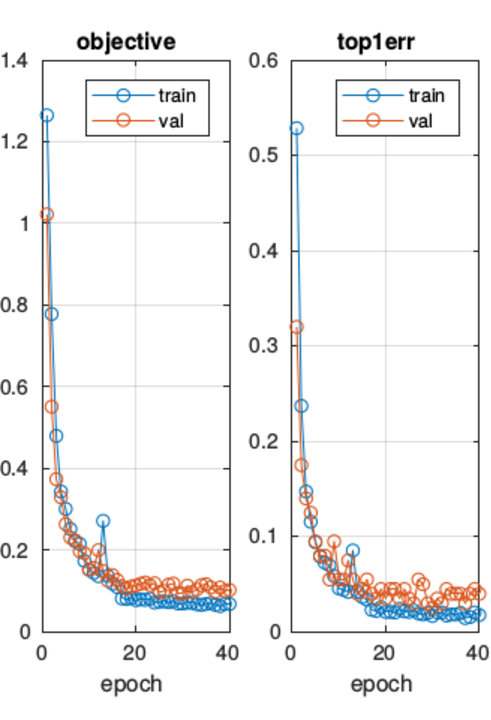
\includegraphics[width=0.3\textwidth]{hw5/imgs/freeze-50-40.jpg}
    }}
\label{fig:augment}
\end{figure}

\section{Conclusion}

In this project we have explored behaviour of BoW approach and CNNs aproach for image classification under different settings.

For BoW approach we have shown that the behaviour is highly dependent on the dataset itself as there are a lot of parameters, which need to be optimized for a specific set of training data. That has been supported by various results for different hyperparameters. That also means, that this algorithm generalizes worse than CNNs. However, we have also shown the ways to optimize hyperparameters in order to achieve better performance.

We have explored how CNNs behave when used for transfer learning, and argued about their advantages over traditional feature extractors, providing empirical results. We have implemented and experimented different variations of the training proecdure, and shown how fine tuning can be harder when using data augmentation, and how freezing layers might lead to lower performance if the features extracted by the pretrained network are not general enough. 

In general, after analyzing how two main approaches for image classification work, we can conclude that there are various improvements that can be done to make algorithms perform better and more efficient, and there is still a lot to innovate in the field of Computer Vision. 

\bibliographystyle{plain}
\bibliography{bibliography}

\end{document}
 